\documentclass{article} % For LaTeX2e
\usepackage{iclr2025_conference,times}

%%%%% NEW MATH DEFINITIONS %%%%%

\usepackage{amsmath,amsfonts,bm}

% Mark sections of captions for referring to divisions of figures
\newcommand{\figleft}{{\em (Left)}}
\newcommand{\figcenter}{{\em (Center)}}
\newcommand{\figright}{{\em (Right)}}
\newcommand{\figtop}{{\em (Top)}}
\newcommand{\figbottom}{{\em (Bottom)}}
\newcommand{\captiona}{{\em (a)}}
\newcommand{\captionb}{{\em (b)}}
\newcommand{\captionc}{{\em (c)}}
\newcommand{\captiond}{{\em (d)}}

% Highlight a newly defined term
\newcommand{\newterm}[1]{{\bf #1}}


% Figure reference, lower-case.
\def\figref#1{figure~\ref{#1}}
% Figure reference, capital. For start of sentence
\def\Figref#1{Figure~\ref{#1}}
\def\twofigref#1#2{figures \ref{#1} and \ref{#2}}
\def\quadfigref#1#2#3#4{figures \ref{#1}, \ref{#2}, \ref{#3} and \ref{#4}}
% Section reference, lower-case.
\def\secref#1{section~\ref{#1}}
% Section reference, capital.
\def\Secref#1{Section~\ref{#1}}
% Reference to two sections.
\def\twosecrefs#1#2{sections \ref{#1} and \ref{#2}}
% Reference to three sections.
\def\secrefs#1#2#3{sections \ref{#1}, \ref{#2} and \ref{#3}}
% Reference to an equation, lower-case.
\def\eqref#1{equation~\ref{#1}}
% Reference to an equation, upper case
\def\Eqref#1{Equation~\ref{#1}}
% A raw reference to an equation---avoid using if possible
\def\plaineqref#1{\ref{#1}}
% Reference to a chapter, lower-case.
\def\chapref#1{chapter~\ref{#1}}
% Reference to an equation, upper case.
\def\Chapref#1{Chapter~\ref{#1}}
% Reference to a range of chapters
\def\rangechapref#1#2{chapters\ref{#1}--\ref{#2}}
% Reference to an algorithm, lower-case.
\def\algref#1{algorithm~\ref{#1}}
% Reference to an algorithm, upper case.
\def\Algref#1{Algorithm~\ref{#1}}
\def\twoalgref#1#2{algorithms \ref{#1} and \ref{#2}}
\def\Twoalgref#1#2{Algorithms \ref{#1} and \ref{#2}}
% Reference to a part, lower case
\def\partref#1{part~\ref{#1}}
% Reference to a part, upper case
\def\Partref#1{Part~\ref{#1}}
\def\twopartref#1#2{parts \ref{#1} and \ref{#2}}

\def\ceil#1{\lceil #1 \rceil}
\def\floor#1{\lfloor #1 \rfloor}
\def\1{\bm{1}}
\newcommand{\train}{\mathcal{D}}
\newcommand{\valid}{\mathcal{D_{\mathrm{valid}}}}
\newcommand{\test}{\mathcal{D_{\mathrm{test}}}}

\def\eps{{\epsilon}}


% Random variables
\def\reta{{\textnormal{$\eta$}}}
\def\ra{{\textnormal{a}}}
\def\rb{{\textnormal{b}}}
\def\rc{{\textnormal{c}}}
\def\rd{{\textnormal{d}}}
\def\re{{\textnormal{e}}}
\def\rf{{\textnormal{f}}}
\def\rg{{\textnormal{g}}}
\def\rh{{\textnormal{h}}}
\def\ri{{\textnormal{i}}}
\def\rj{{\textnormal{j}}}
\def\rk{{\textnormal{k}}}
\def\rl{{\textnormal{l}}}
% rm is already a command, just don't name any random variables m
\def\rn{{\textnormal{n}}}
\def\ro{{\textnormal{o}}}
\def\rp{{\textnormal{p}}}
\def\rq{{\textnormal{q}}}
\def\rr{{\textnormal{r}}}
\def\rs{{\textnormal{s}}}
\def\rt{{\textnormal{t}}}
\def\ru{{\textnormal{u}}}
\def\rv{{\textnormal{v}}}
\def\rw{{\textnormal{w}}}
\def\rx{{\textnormal{x}}}
\def\ry{{\textnormal{y}}}
\def\rz{{\textnormal{z}}}

% Random vectors
\def\rvepsilon{{\mathbf{\epsilon}}}
\def\rvtheta{{\mathbf{\theta}}}
\def\rva{{\mathbf{a}}}
\def\rvb{{\mathbf{b}}}
\def\rvc{{\mathbf{c}}}
\def\rvd{{\mathbf{d}}}
\def\rve{{\mathbf{e}}}
\def\rvf{{\mathbf{f}}}
\def\rvg{{\mathbf{g}}}
\def\rvh{{\mathbf{h}}}
\def\rvu{{\mathbf{i}}}
\def\rvj{{\mathbf{j}}}
\def\rvk{{\mathbf{k}}}
\def\rvl{{\mathbf{l}}}
\def\rvm{{\mathbf{m}}}
\def\rvn{{\mathbf{n}}}
\def\rvo{{\mathbf{o}}}
\def\rvp{{\mathbf{p}}}
\def\rvq{{\mathbf{q}}}
\def\rvr{{\mathbf{r}}}
\def\rvs{{\mathbf{s}}}
\def\rvt{{\mathbf{t}}}
\def\rvu{{\mathbf{u}}}
\def\rvv{{\mathbf{v}}}
\def\rvw{{\mathbf{w}}}
\def\rvx{{\mathbf{x}}}
\def\rvy{{\mathbf{y}}}
\def\rvz{{\mathbf{z}}}

% Elements of random vectors
\def\erva{{\textnormal{a}}}
\def\ervb{{\textnormal{b}}}
\def\ervc{{\textnormal{c}}}
\def\ervd{{\textnormal{d}}}
\def\erve{{\textnormal{e}}}
\def\ervf{{\textnormal{f}}}
\def\ervg{{\textnormal{g}}}
\def\ervh{{\textnormal{h}}}
\def\ervi{{\textnormal{i}}}
\def\ervj{{\textnormal{j}}}
\def\ervk{{\textnormal{k}}}
\def\ervl{{\textnormal{l}}}
\def\ervm{{\textnormal{m}}}
\def\ervn{{\textnormal{n}}}
\def\ervo{{\textnormal{o}}}
\def\ervp{{\textnormal{p}}}
\def\ervq{{\textnormal{q}}}
\def\ervr{{\textnormal{r}}}
\def\ervs{{\textnormal{s}}}
\def\ervt{{\textnormal{t}}}
\def\ervu{{\textnormal{u}}}
\def\ervv{{\textnormal{v}}}
\def\ervw{{\textnormal{w}}}
\def\ervx{{\textnormal{x}}}
\def\ervy{{\textnormal{y}}}
\def\ervz{{\textnormal{z}}}

% Random matrices
\def\rmA{{\mathbf{A}}}
\def\rmB{{\mathbf{B}}}
\def\rmC{{\mathbf{C}}}
\def\rmD{{\mathbf{D}}}
\def\rmE{{\mathbf{E}}}
\def\rmF{{\mathbf{F}}}
\def\rmG{{\mathbf{G}}}
\def\rmH{{\mathbf{H}}}
\def\rmI{{\mathbf{I}}}
\def\rmJ{{\mathbf{J}}}
\def\rmK{{\mathbf{K}}}
\def\rmL{{\mathbf{L}}}
\def\rmM{{\mathbf{M}}}
\def\rmN{{\mathbf{N}}}
\def\rmO{{\mathbf{O}}}
\def\rmP{{\mathbf{P}}}
\def\rmQ{{\mathbf{Q}}}
\def\rmR{{\mathbf{R}}}
\def\rmS{{\mathbf{S}}}
\def\rmT{{\mathbf{T}}}
\def\rmU{{\mathbf{U}}}
\def\rmV{{\mathbf{V}}}
\def\rmW{{\mathbf{W}}}
\def\rmX{{\mathbf{X}}}
\def\rmY{{\mathbf{Y}}}
\def\rmZ{{\mathbf{Z}}}

% Elements of random matrices
\def\ermA{{\textnormal{A}}}
\def\ermB{{\textnormal{B}}}
\def\ermC{{\textnormal{C}}}
\def\ermD{{\textnormal{D}}}
\def\ermE{{\textnormal{E}}}
\def\ermF{{\textnormal{F}}}
\def\ermG{{\textnormal{G}}}
\def\ermH{{\textnormal{H}}}
\def\ermI{{\textnormal{I}}}
\def\ermJ{{\textnormal{J}}}
\def\ermK{{\textnormal{K}}}
\def\ermL{{\textnormal{L}}}
\def\ermM{{\textnormal{M}}}
\def\ermN{{\textnormal{N}}}
\def\ermO{{\textnormal{O}}}
\def\ermP{{\textnormal{P}}}
\def\ermQ{{\textnormal{Q}}}
\def\ermR{{\textnormal{R}}}
\def\ermS{{\textnormal{S}}}
\def\ermT{{\textnormal{T}}}
\def\ermU{{\textnormal{U}}}
\def\ermV{{\textnormal{V}}}
\def\ermW{{\textnormal{W}}}
\def\ermX{{\textnormal{X}}}
\def\ermY{{\textnormal{Y}}}
\def\ermZ{{\textnormal{Z}}}

% Vectors
\def\vzero{{\bm{0}}}
\def\vone{{\bm{1}}}
\def\vmu{{\bm{\mu}}}
\def\vtheta{{\bm{\theta}}}
\def\va{{\bm{a}}}
\def\vb{{\bm{b}}}
\def\vc{{\bm{c}}}
\def\vd{{\bm{d}}}
\def\ve{{\bm{e}}}
\def\vf{{\bm{f}}}
\def\vg{{\bm{g}}}
\def\vh{{\bm{h}}}
\def\vi{{\bm{i}}}
\def\vj{{\bm{j}}}
\def\vk{{\bm{k}}}
\def\vl{{\bm{l}}}
\def\vm{{\bm{m}}}
\def\vn{{\bm{n}}}
\def\vo{{\bm{o}}}
\def\vp{{\bm{p}}}
\def\vq{{\bm{q}}}
\def\vr{{\bm{r}}}
\def\vs{{\bm{s}}}
\def\vt{{\bm{t}}}
\def\vu{{\bm{u}}}
\def\vv{{\bm{v}}}
\def\vw{{\bm{w}}}
\def\vx{{\bm{x}}}
\def\vy{{\bm{y}}}
\def\vz{{\bm{z}}}

% Elements of vectors
\def\evalpha{{\alpha}}
\def\evbeta{{\beta}}
\def\evepsilon{{\epsilon}}
\def\evlambda{{\lambda}}
\def\evomega{{\omega}}
\def\evmu{{\mu}}
\def\evpsi{{\psi}}
\def\evsigma{{\sigma}}
\def\evtheta{{\theta}}
\def\eva{{a}}
\def\evb{{b}}
\def\evc{{c}}
\def\evd{{d}}
\def\eve{{e}}
\def\evf{{f}}
\def\evg{{g}}
\def\evh{{h}}
\def\evi{{i}}
\def\evj{{j}}
\def\evk{{k}}
\def\evl{{l}}
\def\evm{{m}}
\def\evn{{n}}
\def\evo{{o}}
\def\evp{{p}}
\def\evq{{q}}
\def\evr{{r}}
\def\evs{{s}}
\def\evt{{t}}
\def\evu{{u}}
\def\evv{{v}}
\def\evw{{w}}
\def\evx{{x}}
\def\evy{{y}}
\def\evz{{z}}

% Matrix
\def\mA{{\bm{A}}}
\def\mB{{\bm{B}}}
\def\mC{{\bm{C}}}
\def\mD{{\bm{D}}}
\def\mE{{\bm{E}}}
\def\mF{{\bm{F}}}
\def\mG{{\bm{G}}}
\def\mH{{\bm{H}}}
\def\mI{{\bm{I}}}
\def\mJ{{\bm{J}}}
\def\mK{{\bm{K}}}
\def\mL{{\bm{L}}}
\def\mM{{\bm{M}}}
\def\mN{{\bm{N}}}
\def\mO{{\bm{O}}}
\def\mP{{\bm{P}}}
\def\mQ{{\bm{Q}}}
\def\mR{{\bm{R}}}
\def\mS{{\bm{S}}}
\def\mT{{\bm{T}}}
\def\mU{{\bm{U}}}
\def\mV{{\bm{V}}}
\def\mW{{\bm{W}}}
\def\mX{{\bm{X}}}
\def\mY{{\bm{Y}}}
\def\mZ{{\bm{Z}}}
\def\mBeta{{\bm{\beta}}}
\def\mPhi{{\bm{\Phi}}}
\def\mLambda{{\bm{\Lambda}}}
\def\mSigma{{\bm{\Sigma}}}

% Tensor
\DeclareMathAlphabet{\mathsfit}{\encodingdefault}{\sfdefault}{m}{sl}
\SetMathAlphabet{\mathsfit}{bold}{\encodingdefault}{\sfdefault}{bx}{n}
\newcommand{\tens}[1]{\bm{\mathsfit{#1}}}
\def\tA{{\tens{A}}}
\def\tB{{\tens{B}}}
\def\tC{{\tens{C}}}
\def\tD{{\tens{D}}}
\def\tE{{\tens{E}}}
\def\tF{{\tens{F}}}
\def\tG{{\tens{G}}}
\def\tH{{\tens{H}}}
\def\tI{{\tens{I}}}
\def\tJ{{\tens{J}}}
\def\tK{{\tens{K}}}
\def\tL{{\tens{L}}}
\def\tM{{\tens{M}}}
\def\tN{{\tens{N}}}
\def\tO{{\tens{O}}}
\def\tP{{\tens{P}}}
\def\tQ{{\tens{Q}}}
\def\tR{{\tens{R}}}
\def\tS{{\tens{S}}}
\def\tT{{\tens{T}}}
\def\tU{{\tens{U}}}
\def\tV{{\tens{V}}}
\def\tW{{\tens{W}}}
\def\tX{{\tens{X}}}
\def\tY{{\tens{Y}}}
\def\tZ{{\tens{Z}}}


% Graph
\def\gA{{\mathcal{A}}}
\def\gB{{\mathcal{B}}}
\def\gC{{\mathcal{C}}}
\def\gD{{\mathcal{D}}}
\def\gE{{\mathcal{E}}}
\def\gF{{\mathcal{F}}}
\def\gG{{\mathcal{G}}}
\def\gH{{\mathcal{H}}}
\def\gI{{\mathcal{I}}}
\def\gJ{{\mathcal{J}}}
\def\gK{{\mathcal{K}}}
\def\gL{{\mathcal{L}}}
\def\gM{{\mathcal{M}}}
\def\gN{{\mathcal{N}}}
\def\gO{{\mathcal{O}}}
\def\gP{{\mathcal{P}}}
\def\gQ{{\mathcal{Q}}}
\def\gR{{\mathcal{R}}}
\def\gS{{\mathcal{S}}}
\def\gT{{\mathcal{T}}}
\def\gU{{\mathcal{U}}}
\def\gV{{\mathcal{V}}}
\def\gW{{\mathcal{W}}}
\def\gX{{\mathcal{X}}}
\def\gY{{\mathcal{Y}}}
\def\gZ{{\mathcal{Z}}}

% Sets
\def\sA{{\mathbb{A}}}
\def\sB{{\mathbb{B}}}
\def\sC{{\mathbb{C}}}
\def\sD{{\mathbb{D}}}
% Don't use a set called E, because this would be the same as our symbol
% for expectation.
\def\sF{{\mathbb{F}}}
\def\sG{{\mathbb{G}}}
\def\sH{{\mathbb{H}}}
\def\sI{{\mathbb{I}}}
\def\sJ{{\mathbb{J}}}
\def\sK{{\mathbb{K}}}
\def\sL{{\mathbb{L}}}
\def\sM{{\mathbb{M}}}
\def\sN{{\mathbb{N}}}
\def\sO{{\mathbb{O}}}
\def\sP{{\mathbb{P}}}
\def\sQ{{\mathbb{Q}}}
\def\sR{{\mathbb{R}}}
\def\sS{{\mathbb{S}}}
\def\sT{{\mathbb{T}}}
\def\sU{{\mathbb{U}}}
\def\sV{{\mathbb{V}}}
\def\sW{{\mathbb{W}}}
\def\sX{{\mathbb{X}}}
\def\sY{{\mathbb{Y}}}
\def\sZ{{\mathbb{Z}}}

% Entries of a matrix
\def\emLambda{{\Lambda}}
\def\emA{{A}}
\def\emB{{B}}
\def\emC{{C}}
\def\emD{{D}}
\def\emE{{E}}
\def\emF{{F}}
\def\emG{{G}}
\def\emH{{H}}
\def\emI{{I}}
\def\emJ{{J}}
\def\emK{{K}}
\def\emL{{L}}
\def\emM{{M}}
\def\emN{{N}}
\def\emO{{O}}
\def\emP{{P}}
\def\emQ{{Q}}
\def\emR{{R}}
\def\emS{{S}}
\def\emT{{T}}
\def\emU{{U}}
\def\emV{{V}}
\def\emW{{W}}
\def\emX{{X}}
\def\emY{{Y}}
\def\emZ{{Z}}
\def\emSigma{{\Sigma}}

% entries of a tensor
% Same font as tensor, without \bm wrapper
\newcommand{\etens}[1]{\mathsfit{#1}}
\def\etLambda{{\etens{\Lambda}}}
\def\etA{{\etens{A}}}
\def\etB{{\etens{B}}}
\def\etC{{\etens{C}}}
\def\etD{{\etens{D}}}
\def\etE{{\etens{E}}}
\def\etF{{\etens{F}}}
\def\etG{{\etens{G}}}
\def\etH{{\etens{H}}}
\def\etI{{\etens{I}}}
\def\etJ{{\etens{J}}}
\def\etK{{\etens{K}}}
\def\etL{{\etens{L}}}
\def\etM{{\etens{M}}}
\def\etN{{\etens{N}}}
\def\etO{{\etens{O}}}
\def\etP{{\etens{P}}}
\def\etQ{{\etens{Q}}}
\def\etR{{\etens{R}}}
\def\etS{{\etens{S}}}
\def\etT{{\etens{T}}}
\def\etU{{\etens{U}}}
\def\etV{{\etens{V}}}
\def\etW{{\etens{W}}}
\def\etX{{\etens{X}}}
\def\etY{{\etens{Y}}}
\def\etZ{{\etens{Z}}}

% The true underlying data generating distribution
\newcommand{\pdata}{p_{\rm{data}}}
% The empirical distribution defined by the training set
\newcommand{\ptrain}{\hat{p}_{\rm{data}}}
\newcommand{\Ptrain}{\hat{P}_{\rm{data}}}
% The model distribution
\newcommand{\pmodel}{p_{\rm{model}}}
\newcommand{\Pmodel}{P_{\rm{model}}}
\newcommand{\ptildemodel}{\tilde{p}_{\rm{model}}}
% Stochastic autoencoder distributions
\newcommand{\pencode}{p_{\rm{encoder}}}
\newcommand{\pdecode}{p_{\rm{decoder}}}
\newcommand{\precons}{p_{\rm{reconstruct}}}

\newcommand{\laplace}{\mathrm{Laplace}} % Laplace distribution

\newcommand{\E}{\mathbb{E}}
\newcommand{\Ls}{\mathcal{L}}
\newcommand{\R}{\mathbb{R}}
\newcommand{\emp}{\tilde{p}}
\newcommand{\lr}{\alpha}
\newcommand{\reg}{\lambda}
\newcommand{\rect}{\mathrm{rectifier}}
\newcommand{\softmax}{\mathrm{softmax}}
\newcommand{\sigmoid}{\sigma}
\newcommand{\softplus}{\zeta}
\newcommand{\KL}{D_{\mathrm{KL}}}
\newcommand{\Var}{\mathrm{Var}}
\newcommand{\standarderror}{\mathrm{SE}}
\newcommand{\Cov}{\mathrm{Cov}}
% Wolfram Mathworld says $L^2$ is for function spaces and $\ell^2$ is for vectors
% But then they seem to use $L^2$ for vectors throughout the site, and so does
% wikipedia.
\newcommand{\normlzero}{L^0}
\newcommand{\normlone}{L^1}
\newcommand{\normltwo}{L^2}
\newcommand{\normlp}{L^p}
\newcommand{\normmax}{L^\infty}

\newcommand{\parents}{Pa} % See usage in notation.tex. Chosen to match Daphne's book.

\DeclareMathOperator*{\argmax}{arg\,max}
\DeclareMathOperator*{\argmin}{arg\,min}

\DeclareMathOperator{\sign}{sign}
\DeclareMathOperator{\Tr}{Tr}
\let\ab\allowbreak


\usepackage{hyperref}
\usepackage{url}
\usepackage{graphicx}
\usepackage{booktabs}
\usepackage{amsmath}
\usepackage{xcolor}

\title{Learning to Search the Literature: \\
Budgeted Citation-Graph Agents for Systematic Review \\
\large Midway Report}

\author{Katherine Xu \\
Stanford University \\
\texttt{kwx04@stanford.edu} \\
\url{https://github.com/katherinewxu/literature-search-agent}}

\iclrfinalcopy % Uncomment for camera-ready version, but NOT for submission.
\begin{document}

\maketitle
\lhead{CS329Z Midway Report, Stanford University}
\thispagestyle{fancy}

\section{Research Questions}

Systematic reviews depend on a search that finds every eligible study, and a missed study can
change a review's conclusion. We study literature search as a budgeted sequential decision
problem: given a review's question and eligibility criteria, an agent spends a fixed number of
tool calls on keyword search, citation chasing and reading, and is scored on how many of the
review's included studies it recovers. We ask four questions.
\textbf{(Q1)} At equal budget, do prompted LLM agents beat retrieval and scripted snowballing
baselines?
\textbf{(Q2)} Can a small open model trained with supervised fine-tuning and reinforcement learning
match or beat a much larger prompted model?
\textbf{(Q3)} Which strategies emerge: how do agents divide their budget between search and
citation chasing, and when do they stop?
\textbf{(Q4)} Do the results transfer to reviews from other fields?
Proposal feedback added a further question: is the citation graph itself limiting, and would
open-web search help? The results raised one more: \textbf{(Q5)} can an agent tell how much it has
missed, i.e.\ estimate its own recall when it stops?

\section{Environment \& Data}

\textbf{Data.} Gold sets come from SYNERGY+ \citep{debruin2023synergy}: 72 published systematic
reviews, each with the candidate papers its authors screened and the subset they included (the
gold set $R$). Metadata, abstracts and the citation graph come from OpenAlex
\citep{priem2022openalex} and are frozen into a local store, so episodes run offline and are
reproducible. Splits are by review (Table~\ref{tab:splits}). The 8 evaluation reviews are fixed
for all systems and themselves split train/dev/test; the only tuned baseline parameter was chosen
on the train reviews. The 24 transfer reviews come from fields that do not appear in training.

\begin{table}[h]
\centering
\small
\begin{tabular}{@{}p{0.13\linewidth}p{0.2\linewidth}p{0.27\linewidth}p{0.30\linewidth}@{}}
\toprule
set & reviews & fields & used for \\
\midrule
evaluation & 8 (4 train / 2 dev / 2 test) & life science & all systems \\
training & 40 & life science & teacher trajectories, SFT, GRPO; extra evaluation of prompted systems \\
transfer & 24 & software eng., education, psychology, \dots & out-of-field evaluation \\
\bottomrule
\end{tabular}
\caption{Review splits. The sets are disjoint. The proposal also listed CLEF TAR and CSMeD;
SYNERGY+ alone provided enough reviews, so we did not add them.}
\label{tab:splits}
\end{table}

\textbf{Environment.} Each episode is a partially observed decision process. The agent observes
the review question, the eligibility criteria, its remaining budget $B$, the latest tool result,
a frontier of the 50 most recently seen papers, and its included and excluded sets. Episodes start
from five seed papers found by BM25 \citep{robertson2009bm25} on the question and criteria. Each
turn the agent may screen any paper it has seen (include or exclude, free) and take one paid
action:
\texttt{search(query, k$\le$10)}, which costs 1 and returns the top unseen BM25 results (repeating
a query pages deeper);
\texttt{expand\_refs(p)} and \texttt{expand\_citers(p)}, which cost 1 per 10 results ($k\le 20$)
and return a paper's references or citers;
\texttt{read(p)}, which costs 1 and returns the abstract; and \texttt{stop}. Budgets are
$B\in\{10, 20, 40\}$, and there are three tool sets: \emph{keyword} (search only),
\emph{citation} (expansion only) and \emph{hybrid} (both). Once the budget is spent the agent may
still screen what it has seen.

\textbf{Leakage control.} The review paper, every paper that cites it, and every paper published
after it are hidden from the agent. Gold labels are used only by the scorer, never in prompts,
seeds or queries, and an automated leakage audit was run on the training data before any training.

\textbf{Search universes.} To test whether the graph is limiting, the same agents run in three
universes of increasing size:
(i) the \emph{closed pool}, the papers the review authors screened;
(ii) the \emph{open graph}, the pool plus up to 5{,}000 papers it cites, roughly doubling the
distractors; and
(iii) \emph{live web}, all of OpenAlex ($\sim$250M works), with search, references and citers
served by the live API and cached for replay.

\textbf{Metrics and success criteria.} The primary metric is recall $|S\cap R|/|R|$ of the
included set $S$ at each budget. We also report precision and F1 of $S$, the area under the
recall-versus-cost curve, and the action mix. Comparisons are paired by review, with 95\%
bootstrap confidence intervals over reviews and win/loss counts. A system ``beats'' another only
when the interval excludes zero. The training reward is
$r = |S\cap R|/|R| - \lambda\,|S\setminus R|/|S|$ with $\lambda = 0.1$.

\section{Methods}

\textbf{Baselines.} (1) \emph{BM25} and (2) \emph{SPECTER2} \citep{singh2023scirepeval} rank the
pool against the review text and include every result the budget pays for. This is the recall a
retriever reaches without screening, at the lowest possible precision. (3) A scripted
\emph{snowball} agent searches, screens by keyword overlap, and chases the references and citers
of included papers \citep{wohlin2014snowballing}. (4) A \emph{random} traversal.

\textbf{Prompted agents.} One prompt and one tool protocol for every model. Each turn the model
returns JSON with screening decisions and exactly one action; invalid actions are charged and
logged. Models: Claude Sonnet 5.5 and Haiku 5.5, and Qwen3-32B \citep{yang2025qwen3}, at
temperature 0 via OpenRouter, with a hard spending cap enforced in code.

\textbf{Trained agent (focus of the investigation).} Qwen3-1.7B with LoRA
\citep{hu2022lora}, trained in two stages after a pre-registered gate was met: at least 200
valid teacher trajectories (we had 360), a passing leakage audit, and a one-GPU smoke test.
\emph{SFT}: rejection sampling keeps the better half (by reward) of Haiku 5.5 trajectories on the
40 training reviews, giving 2{,}702 turns; 337 steps on one L40S.
\emph{GRPO} \citep{shao2024deepseekmath}: starting from the SFT adapter, groups of 8 rollouts
per task, KL penalty to SFT ($\beta=0.02$), 40 steps at $B=20$ over all three tool sets.
Rollouts and evaluation are served with vLLM \citep{kwon2023vllm}. Both stages were repeated
with a second seed. The open question for the rest of the quarter is what RL adds beyond
imitation, and whether a trained policy learns to use citation tools at all.

\section{Summary of Progress}

\textbf{Done.}
\begin{itemize}
\item The environment, all baselines, the prompted agents and the training pipeline are
  implemented and tested (54 unit tests, including leakage and cost-accounting tests).
\item Every system has been run on the 8 evaluation reviews $\times$ 3 tool sets $\times$ 3
  budgets, in both the closed pool and the open graph, and on the 24 transfer reviews. The
  prompted systems were also run on the 40 training reviews, so their life-science comparisons
  rest on 48 reviews.
\item Robustness checks:
  \begin{itemize}
  \item three temperature-0.7 repeats for the API models;
  \item a closed-book memorization probe, with all systems rescored after removing every gold
    paper any model could name from memory;
  \item a second training seed;
  \item an agent that uses SPECTER2 as its search tool.
  \end{itemize}
\item A step-by-step HTML replay of episodes, for the demo.
\end{itemize}

\begin{figure}[t]
\centering
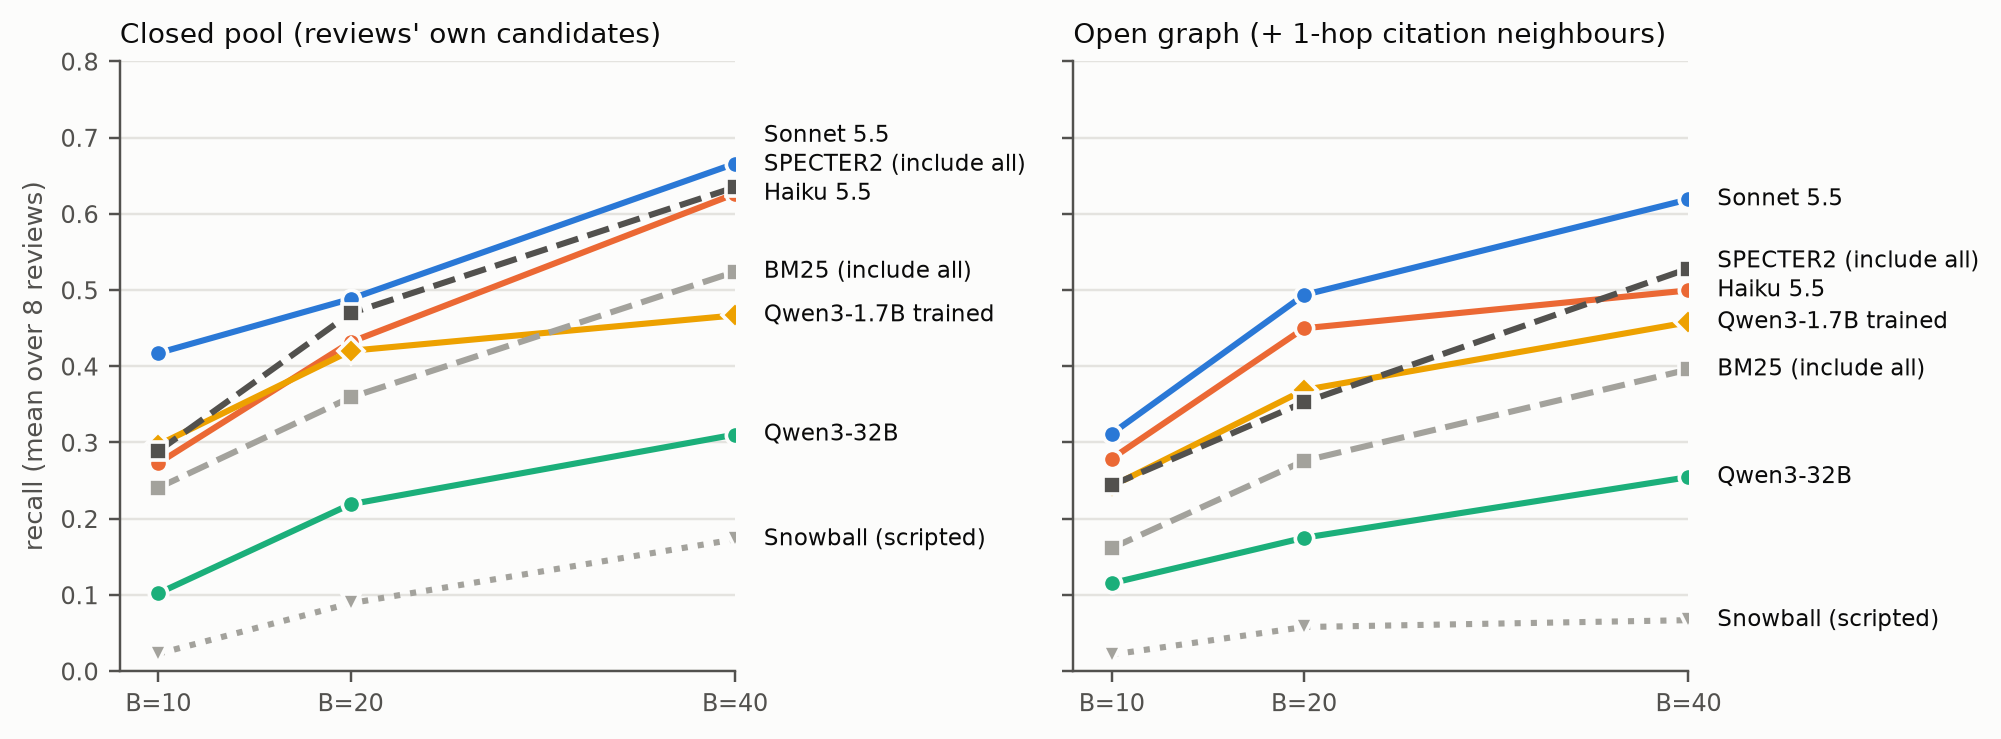
\includegraphics[width=\linewidth]{figures/fig1_recall_vs_budget.png}
\caption{Recall by budget with hybrid tools, mean over the 8 evaluation reviews. Left: closed
pool. Right: open graph. Dashed lines are retrieval baselines that include everything they
see.}
\label{fig:budget}
\end{figure}

\textbf{Preliminary results.} Recall at $B=40$ with hybrid tools; brackets are 95\% CIs of the
paired difference.

\begin{itemize}
\item \textbf{Q1.} Sonnet beats BM25 by $+.152$ $[+.07, +.23]$ on 48 life-science reviews and by
  $+.087$ $[+.01, +.16]$ on the 24 transfer reviews. Its precision is about 8$\times$ higher (.42
  vs.\ .05).
  \begin{itemize}
  \item The scripted snowball loses to Sonnet on 8 of 8 reviews at every budget.
  \item Exhaustive SPECTER2 is the strongest baseline: its recall ties Sonnet's in the closed
    pool ($+.031$ $[-.05, +.12]$), but its precision is only .06.
  \end{itemize}
\item \textbf{Q2.} SFT moves the 1.7B model from .13 to .43 recall (closed pool); no review
  gets worse.
  \begin{itemize}
  \item The trained model beats prompted Qwen3-32B by $+.133$ $[+.08, +.19]$ on transfer.
  \item It matches its Haiku teacher out of field ($+.007$), but trails it in field ($-.159$).
  \item GRPO adds $+.01$ to $+.07$ over SFT in all six seed $\times$ condition cells. Seed-to-seed
    variation is about as large.
  \item \emph{GRPO v2} (F$_2$ reward, turn-level credit from each call's marginal gold gain with a
    redundancy penalty, in the spirit of PaSa's per-call reward \citep{he2025pasa}, mixed budgets,
    120 steps; two seeds plus an ablation without turn credit) missed its pre-stated criteria: at
    $B\ge 20$ no run reached precision $\ge .25$ with recall within .02 of v1, and its recall gain
    over SFT was not consistently beyond seed noise. Turn credit trades recall for precision
    (transfer, $B=40$: recall $-.052$ $[-.10, -.01]$, precision $+.062$ $[+.05, +.08]$, F1 $+.042$
    $[+.02, +.06]$), and with hybrid tools the policy still spends all its budget on search.
  \item Exploratory: with citation tools only, v2 stops early less often (20--28 of 40 calls spent,
    vs.\ about 8 for SFT), and recall rises by $+.09$ to $+.24$ over SFT in all six seed
    $\times$ universe cells on 8 reviews. Absolute recall stays low (.13--.30).
  \end{itemize}
\item \textbf{Q3.} Given both tools, frontier agents spend 80--90\% of the budget on new
  queries and almost none on citation chasing; the trained model re-pages a dozen queries.
  With citation tools only, every model stops early (Sonnet leaves half of $B=40$ unused).
\item \textbf{Graph question.} Opening the graph lowers every system's recall (Sonnet
  .67$\to$.62, BM25 .52$\to$.40), although 77--100\% of gold lies within three hops of the
  seeds. The budget and the off-topic papers it must pay for limit the agents, not graph
  connectivity.
\item \textbf{Live web.} On all of OpenAlex, Sonnet's recall falls from .67 to .32 and Haiku's
  from .63 to .17. Raw OpenAlex search finds 1\% of gold, so the LLM's lead over include-all
  retrieval grows from $+.14$ (closed) to $+.22$ (open graph) to $+.31$ (web). On the 24 transfer
  reviews Haiku falls from .48 to .10 ($-.379$ $[-.47, -.30]$), still ahead of raw search (.02) by
  $+.080$ $[+.06, +.11]$.
\item \textbf{Forced citation chasing.} Replacing every third action with expansion of a paper
  the agent already included lowers recall (Haiku $-.097$ $[-.19, -.02]$ closed, $-.071$
  $[-.12, -.03]$ on 24 transfer reviews; Sonnet $-.018$, n.s.; trained 1.7B $-.064$ $[-.12, -.01]$
  at $B=20$, $-.003$ at $B=40$). Unlike PaSa \citep{he2025pasa}, in our setting citation hops are a
  poor use of budget.
\item \textbf{Q5.} End-of-episode recall estimates rank episodes ($r\approx .5$--$.7$) but are
  inaccurate per episode (error $\approx .2$). An LLM screener cannot audit the agent: it accepts
  92\% of gold but also 87\% of the agent's false inclusions.
\item \textbf{Checks.} Removing memorized gold (7\% of closed-pool gold) changes no system's
  recall by more than .02.
\end{itemize}

\textbf{Still to do.}
\begin{itemize}
\item Test whether larger budgets (100--400 calls) change the search-versus-citation result, and
  how close recall gets to the level real reviews need.
\item Tighten the end-of-episode recall bound (mean lower bound is only about .15).
\item Hand-label a sample of ``false positives'' to estimate how often agents find eligible
  studies missing from the gold set, as proposed.
\item Write a fuller error analysis by failure type: premature stopping, reachable but not
  reached, screened out, missing abstract.
\item Write the related-work section, the live demo, and a README quick-start that runs one
  episode on a small subgraph with the released checkpoint.
\item Try the refutation-reward variant if time allows (stretch goal).
\end{itemize}

\textbf{Obstacles and concerns.}
\begin{itemize}
\item \textbf{OpenAlex request limits.} The key allows about 1{,}000 searches a day, so the
  live-web runs are paced across days.
\item \textbf{API spending.} About \$55 of the \$60 project cap is spent, leaving little room for new
  frontier-model runs.
\item \textbf{Small in-field test set for the trained model.} Its 40 training reviews cannot be
  reused, so its in-field claims rest on 8 reviews. Its transfer claims rest on 24.
\item \textbf{Training variance.} Two seeds differ by up to .07 recall, as much as the GRPO
  effect, so ranking training recipes will need more seeds.
\item \textbf{Missing abstracts.} About a quarter of gold papers lack an OpenAlex abstract,
  which caps screening accuracy for every system.
\end{itemize}

\bibliography{references}
\bibliographystyle{iclr2025_conference}

\appendix
\section{AI-Use Disclosure Statement}

\textcolor{red}{[DRAFT: Katherine, check this against what you actually did and edit before
submitting.]}
\textbf{Ideation.} The research questions and formulation come from my proposal, written by me
with the limited assistance described in its own disclosure.
\textbf{Code and experiments.} I used Claude Code (Anthropic), an AI coding agent, extensively.
Under my direction it wrote most of the implementation: environment, baselines, LLM agent,
training scripts, analysis scripts and tests. It also ran the experiments on Stanford FarmShare
and computed the analyses and figures. I set the research questions, the evaluation protocol,
the pre-registered training gate and the spending limits, and I reviewed the results.
\textbf{Writing.} Claude Code drafted this report from the experiment logs. I revised it and am
responsible for every claim in it. The LLM agents studied in this project (Claude Sonnet 5.5,
Claude Haiku 5.5, Qwen3) are the objects of study, not authors.

\end{document}
